\chapter{Virtauslaskenta}

Virtauslaskenta on verkkoteorian osa-alue,
joka tutkii verkossa kulkevia virtauksia.
Keskeinen virtauslaskennan ongelma on
laskea maksimivirtaus kahden verkon solmun välillä.
Maksimivirtausta voi soveltaa
monissa verkko-on\-gel\-mis\-sa,
kuten maksimiparituksen ja
minimileikkauksen laskemisessa.

\section{Käsitteitä}

Tämän luvun algoritmit käsittelevät suunnattua, painotettua
verkkoa, jossa on valittu alkusolmu ja loppusolmu.
Määrittelemme seuraavaksi kaksi käsitettä, jotka 
ovat saman asian kaksi eri puolta.

Käytämme esimerkkinä seuraavaa verkkoa,
jossa solmu 1 on alkusolmu ja solmu 6 on loppusolmu:

\begin{center}
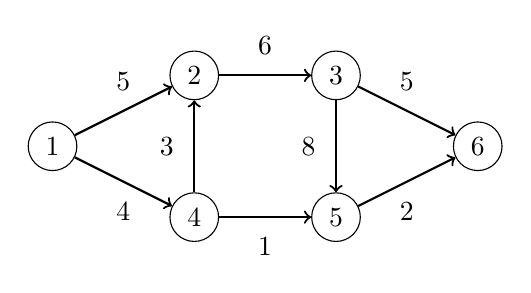
\begin{tikzpicture}[scale=0.9]
\node[draw, circle] (1) at (1,2) {$1$};
\node[draw, circle] (2) at (3,3) {$2$};
\node[draw, circle] (3) at (5,3) {$3$};
\node[draw, circle] (4) at (7,2) {$6$};
\node[draw, circle] (5) at (3,1) {$4$};
\node[draw, circle] (6) at (5,1) {$5$};
\path[draw,thick,->] (1) -- node[font=\small,label=5] {} (2);
\path[draw,thick,->] (2) -- node[font=\small,label=6] {} (3);
\path[draw,thick,->] (3) -- node[font=\small,label=5] {} (4);
\path[draw,thick,->] (1) -- node[font=\small,label=below:4] {} (5);
\path[draw,thick,->] (5) -- node[font=\small,label=below:1] {} (6);
\path[draw,thick,->] (6) -- node[font=\small,label=below:2] {} (4);
\path[draw,thick,<-] (2) -- node[font=\small,label=left:3] {} (5);
\path[draw,thick,->] (3) -- node[font=\small,label=left:8] {} (6);
\end{tikzpicture}
\end{center}

\subsubsection{Maksimivirtaus}

Maksimivirtaus (\textit{maximum flow}) on suurin
mahdollinen virtaus,
joka lähtee liikkeelle alkusolmusta,
päätyy loppusolmuun eikä ylitä minkään
kaaren kapasiteettia (painoa).
Kaikissa solmuissa alku- ja loppusolmua
lukuun ottamatta tulevan ja lähtevän
virtauksen tulee olla sama.

Esimerkkiverkon maksimivirtaus on 7,
joka muodostuu seuraavasti:

\begin{center}
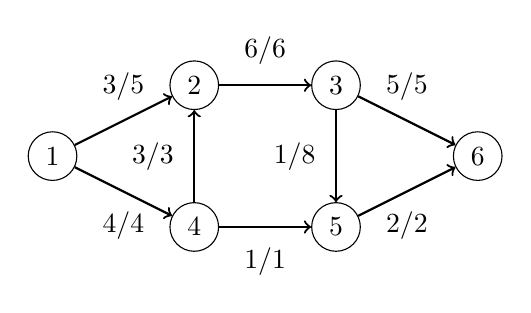
\begin{tikzpicture}[scale=0.9]
\node[draw, circle] (1) at (1,2) {$1$};
\node[draw, circle] (2) at (3,3) {$2$};
\node[draw, circle] (3) at (5,3) {$3$};
\node[draw, circle] (4) at (7,2) {$6$};
\node[draw, circle] (5) at (3,1) {$4$};
\node[draw, circle] (6) at (5,1) {$5$};
\path[draw,thick,->] (1) -- node[font=\small,label=3/5] {} (2);
\path[draw,thick,->] (2) -- node[font=\small,label=6/6] {} (3);
\path[draw,thick,->] (3) -- node[font=\small,label=5/5] {} (4);
\path[draw,thick,->] (1) -- node[font=\small,label=below:4/4] {} (5);
\path[draw,thick,->] (5) -- node[font=\small,label=below:1/1] {} (6);
\path[draw,thick,->] (6) -- node[font=\small,label=below:2/2] {} (4);
\path[draw,thick,<-] (2) -- node[font=\small,label=left:3/3] {} (5);
\path[draw,thick,->] (3) -- node[font=\small,label=left:1/8] {} (6);
\end{tikzpicture}
\end{center}

Merkintä $v/k$ kaaressa tarkoittaa,
että kaaressa kulkee virtausta $v$
ja kaaren kapasiteetti on $k$.
Virtauksen suuruus on 7, koska alkusolmusta
lähtevä virtaus on $3+4=7$ ja loppusolmuun
saapuva virtaus on $5+2=7$.
Virtaus on maksimivirtaus, koska ei ole tapaa
lähettää enempää virtausta verkossa.

\subsubsection{Minimileikkaus}

Minimileikkaus (\textit{minimum cut}) jakaa verkon
kahteen osaan niin, että alkusolmu ja loppusolmu
ovat eri osissa ja alkusolmun osasta
loppusolmun osaan kulkevien kaarten painojen
summa on pienin mahdollinen.

Esimerkkiverkossa minimileikkaus on painoltaan 7:

\begin{center}
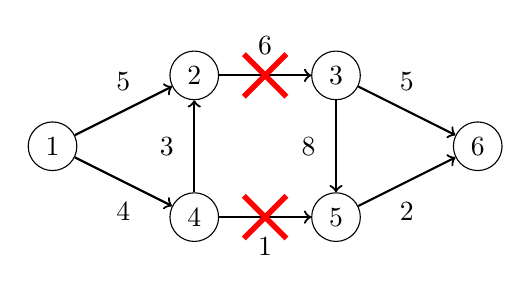
\begin{tikzpicture}[scale=0.9]
\node[draw, circle] (1) at (1,2) {$1$};
\node[draw, circle] (2) at (3,3) {$2$};
\node[draw, circle] (3) at (5,3) {$3$};
\node[draw, circle] (4) at (7,2) {$6$};
\node[draw, circle] (5) at (3,1) {$4$};
\node[draw, circle] (6) at (5,1) {$5$};
\path[draw,thick,->] (1) -- node[font=\small,label=5] {} (2);
\path[draw,thick,->] (2) -- node[font=\small,label=6] {} (3);
\path[draw,thick,->] (3) -- node[font=\small,label=5] {} (4);
\path[draw,thick,->] (1) -- node[font=\small,label=below:4] {} (5);
\path[draw,thick,->] (5) -- node[font=\small,label=below:1] {} (6);
\path[draw,thick,->] (6) -- node[font=\small,label=below:2] {} (4);
\path[draw,thick,<-] (2) -- node[font=\small,label=left:3] {} (5);
\path[draw,thick,->] (3) -- node[font=\small,label=left:8] {} (6);

\path[draw=red,thick,-,line width=2pt] (4-.3,3-.3) -- (4+.3,3+.3);
\path[draw=red,thick,-,line width=2pt] (4-.3,3+.3) -- (4+.3,3-.3);
\path[draw=red,thick,-,line width=2pt] (4-.3,1-.3) -- (4+.3,1+.3);
\path[draw=red,thick,-,line width=2pt] (4-.3,1+.3) -- (4+.3,1-.3);
\end{tikzpicture}
\end{center}

Tässä alkusolmun osassa ovat solmut $\{1,2,4\}$
ja loppusolmun osassa ovat solmut $\{3,5,6\}$.
Alkusolmun osasta loppusolmun osaan kulkevat
kaaret $2 \rightarrow 3$ ja $4 \rightarrow 5$,
joiden yhteispaino on $6+1=7$.

~\\
\noindent
Ei ole sattumaa, että yllä olevassa verkossa
maksimivirtaus ja minimileikkaus ovat yhtä suuret.
Seuraavaksi tutustumme algoritmiin, jonka avulla
voi määrittää verkon maksimivirtauksen,
minkä jälkeen näemme, miksi maksimivirtaus on
aina yhtä suuri kuin minimileikkaus.

\section{Ford-Fulkersonin algoritmi}

Ford-Fulkersonin algoritmi etsii verkon maksimivirtauksen.
Algoritmin ideana on aloittaa tilanteesta,
jossa virtaus on 0, ja etsiä sitten verkosta polkuja,
jotka tuottavat siihen lisää virtausta.
Kun mitään polkua ei enää pysty muodostamaan,
maksimivirtaus on valmis.

Algoritmi käsittelee verkkoa muodossa,
jossa jokaiselle kaarelle on vastakkaiseen
suuntaan kulkeva pari.
Kaaren paino kuvastaa, miten paljon
lisää virtausta sen kautta pystyisi vielä kulkemaan.
Aluksi alkuperäisen verkon kaarilla on
painona niiden kapasiteetti
ja lisätyillä kaarilla on painona 0.

Esimerkkiverkosta syntyy seuraava verkko:

\begin{center}
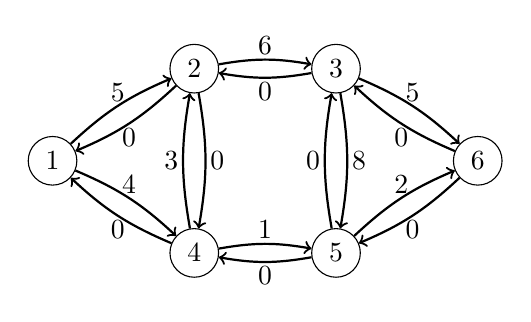
\begin{tikzpicture}[scale=0.9,label distance=-2mm]
\node[draw, circle] (1) at (1,1.3) {$1$};
\node[draw, circle] (2) at (3,2.6) {$2$};
\node[draw, circle] (3) at (5,2.6) {$3$};
\node[draw, circle] (4) at (7,1.3) {$6$};
\node[draw, circle] (5) at (3,0) {$4$};
\node[draw, circle] (6) at (5,0) {$5$};

\path[draw,thick,->] (1) edge [bend left=10] node[font=\small,label=5] {} (2);
\path[draw,thick,->] (2) edge [bend left=10] node[font=\small,label=below:0] {} (1);
\path[draw,thick,->] (2) edge [bend left=10] node[font=\small,label=6] {} (3);
\path[draw,thick,->] (3) edge [bend left=10] node[font=\small,label=below:0] {} (2);
\path[draw,thick,->] (3) edge [bend left=10] node[font=\small,label=5] {} (4);
\path[draw,thick,->] (4) edge [bend left=10] node[font=\small,label=below:0] {} (3);
\path[draw,thick,->] (1) edge [bend left=10] node[font=\small,label=4] {} (5);
\path[draw,thick,->] (5) edge [bend left=10] node[font=\small,label=below:0] {} (1);
\path[draw,thick,->] (5) edge [bend left=10] node[font=\small,label=1] {} (6);
\path[draw,thick,->] (6) edge [bend left=10] node[font=\small,label=below:0] {} (5);
\path[draw,thick,->] (6) edge [bend left=10] node[font=\small,label=2] {} (4);
\path[draw,thick,->] (4) edge [bend left=10] node[font=\small,label=below:0] {} (6);
\path[draw,thick,->] (5) edge [bend left=10] node[font=\small,label=left:3] {} (2);
\path[draw,thick,->] (2) edge [bend left=10] node[font=\small,label=right:0] {} (5);
\path[draw,thick,->] (3) edge [bend left=10] node[font=\small,label=right:8] {} (6);
\path[draw,thick,->] (6) edge [bend left=10] node[font=\small,label=left:0] {} (3);
\end{tikzpicture}
\end{center}

\subsubsection{Algoritmin toiminta}

Ford-Fulkersonin algoritmi etsii verkosta joka vaiheessa polun,
joka alkaa alkusolmusta,
päättyy loppusolmuun ja jossa jokaisen kaaren
paino on positiivinen.
Jos vaihtoehtoja on useita, mikä tahansa valinta kelpaa.

Esimerkkiverkossa voimme valita vaikkapa seuraavan polun:

\begin{center}
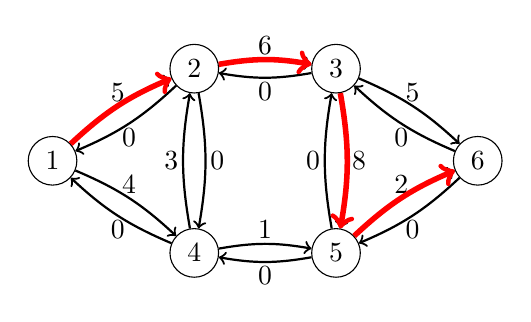
\begin{tikzpicture}[scale=0.9,label distance=-2mm]
\node[draw, circle] (1) at (1,1.3) {$1$};
\node[draw, circle] (2) at (3,2.6) {$2$};
\node[draw, circle] (3) at (5,2.6) {$3$};
\node[draw, circle] (4) at (7,1.3) {$6$};
\node[draw, circle] (5) at (3,0) {$4$};
\node[draw, circle] (6) at (5,0) {$5$};

\path[draw,thick,->] (1) edge [bend left=10] node[font=\small,label=5] {} (2);
\path[draw,thick,->] (2) edge [bend left=10] node[font=\small,label=below:0] {} (1);
\path[draw,thick,->] (2) edge [bend left=10] node[font=\small,label=6] {} (3);
\path[draw,thick,->] (3) edge [bend left=10] node[font=\small,label=below:0] {} (2);
\path[draw,thick,->] (3) edge [bend left=10] node[font=\small,label=5] {} (4);
\path[draw,thick,->] (4) edge [bend left=10] node[font=\small,label=below:0] {} (3);
\path[draw,thick,->] (1) edge [bend left=10] node[font=\small,label=4] {} (5);
\path[draw,thick,->] (5) edge [bend left=10] node[font=\small,label=below:0] {} (1);
\path[draw,thick,->] (5) edge [bend left=10] node[font=\small,label=1] {} (6);
\path[draw,thick,->] (6) edge [bend left=10] node[font=\small,label=below:0] {} (5);
\path[draw,thick,->] (6) edge [bend left=10] node[font=\small,label=2] {} (4);
\path[draw,thick,->] (4) edge [bend left=10] node[font=\small,label=below:0] {} (6);
\path[draw,thick,->] (5) edge [bend left=10] node[font=\small,label=left:3] {} (2);
\path[draw,thick,->] (2) edge [bend left=10] node[font=\small,label=right:0] {} (5);
\path[draw,thick,->] (3) edge [bend left=10] node[font=\small,label=right:8] {} (6);
\path[draw,thick,->] (6) edge [bend left=10] node[font=\small,label=left:0] {} (3);

\path[draw=red,thick,->,line width=2pt] (1) edge [bend left=10] (2);
\path[draw=red,thick,->,line width=2pt] (2) edge [bend left=10] (3);
\path[draw=red,thick,->,line width=2pt] (3) edge [bend left=10] (6);
\path[draw=red,thick,->,line width=2pt] (6) edge [bend left=10] (4);
\end{tikzpicture}
\end{center}

Polun valinnan jälkeen virtaus lisääntyy $v$ yksikköä,
jossa $v$ on pienin kaaren paino polulla.
Samalla jokaisen polun osana olevan kaaren paino
laskee $v$:llä ja jokaisen vastakkaiseen suuntaan
kulkevan kaaren paino nousee $v$:llä.

Yllä valitussa polussa pienin kaaren paino on 2,
joten virtaus kasvaa 2:lla
ja verkko muuttuu seuraavasti:

\begin{center}
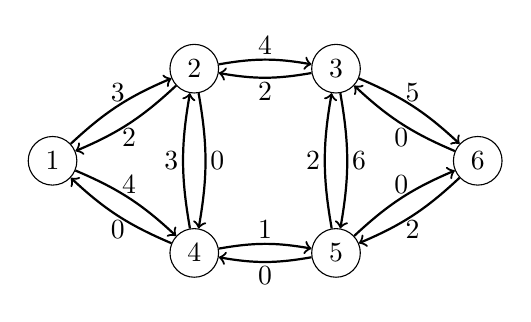
\begin{tikzpicture}[scale=0.9,label distance=-2mm]
\node[draw, circle] (1) at (1,1.3) {$1$};
\node[draw, circle] (2) at (3,2.6) {$2$};
\node[draw, circle] (3) at (5,2.6) {$3$};
\node[draw, circle] (4) at (7,1.3) {$6$};
\node[draw, circle] (5) at (3,0) {$4$};
\node[draw, circle] (6) at (5,0) {$5$};

\path[draw,thick,->] (1) edge [bend left=10] node[font=\small,label=3] {} (2);
\path[draw,thick,->] (2) edge [bend left=10] node[font=\small,label=below:2] {} (1);
\path[draw,thick,->] (2) edge [bend left=10] node[font=\small,label=4] {} (3);
\path[draw,thick,->] (3) edge [bend left=10] node[font=\small,label=below:2] {} (2);
\path[draw,thick,->] (3) edge [bend left=10] node[font=\small,label=5] {} (4);
\path[draw,thick,->] (4) edge [bend left=10] node[font=\small,label=below:0] {} (3);
\path[draw,thick,->] (1) edge [bend left=10] node[font=\small,label=4] {} (5);
\path[draw,thick,->] (5) edge [bend left=10] node[font=\small,label=below:0] {} (1);
\path[draw,thick,->] (5) edge [bend left=10] node[font=\small,label=1] {} (6);
\path[draw,thick,->] (6) edge [bend left=10] node[font=\small,label=below:0] {} (5);
\path[draw,thick,->] (6) edge [bend left=10] node[font=\small,label=0] {} (4);
\path[draw,thick,->] (4) edge [bend left=10] node[font=\small,label=below:2] {} (6);
\path[draw,thick,->] (5) edge [bend left=10] node[font=\small,label=left:3] {} (2);
\path[draw,thick,->] (2) edge [bend left=10] node[font=\small,label=right:0] {} (5);
\path[draw,thick,->] (3) edge [bend left=10] node[font=\small,label=right:6] {} (6);
\path[draw,thick,->] (6) edge [bend left=10] node[font=\small,label=left:2] {} (3);
\end{tikzpicture}
\end{center}

Muutoksessa on ideana, että virtauksen lisääminen
vähentää polkuun kuuluvien kaarten kykyä välittää virtausta.
Toisaalta virtausta on mahdollista peruuttaa myöhemmin
käyttämällä vastakkaiseen suuntaan meneviä kaaria.

Algoritmi lisää virtausta pikkuhiljaa
niin kauan, kuin polkuja alkusolmusta loppusolmuun
on olemassa.
Esimerkissä seuraava polku voisi olla vaikkapa:

\begin{center}
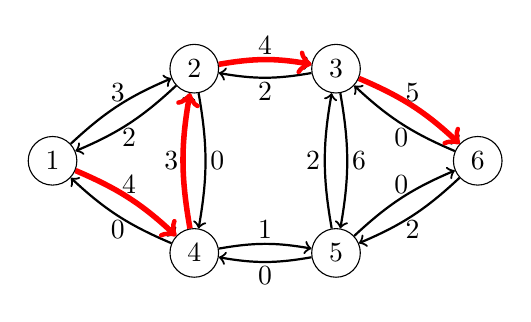
\begin{tikzpicture}[scale=0.9,label distance=-2mm]
\node[draw, circle] (1) at (1,1.3) {$1$};
\node[draw, circle] (2) at (3,2.6) {$2$};
\node[draw, circle] (3) at (5,2.6) {$3$};
\node[draw, circle] (4) at (7,1.3) {$6$};
\node[draw, circle] (5) at (3,0) {$4$};
\node[draw, circle] (6) at (5,0) {$5$};

\path[draw,thick,->] (1) edge [bend left=10] node[font=\small,label=3] {} (2);
\path[draw,thick,->] (2) edge [bend left=10] node[font=\small,label=below:2] {} (1);
\path[draw,thick,->] (2) edge [bend left=10] node[font=\small,label=4] {} (3);
\path[draw,thick,->] (3) edge [bend left=10] node[font=\small,label=below:2] {} (2);
\path[draw,thick,->] (3) edge [bend left=10] node[font=\small,label=5] {} (4);
\path[draw,thick,->] (4) edge [bend left=10] node[font=\small,label=below:0] {} (3);
\path[draw,thick,->] (1) edge [bend left=10] node[font=\small,label=4] {} (5);
\path[draw,thick,->] (5) edge [bend left=10] node[font=\small,label=below:0] {} (1);
\path[draw,thick,->] (5) edge [bend left=10] node[font=\small,label=1] {} (6);
\path[draw,thick,->] (6) edge [bend left=10] node[font=\small,label=below:0] {} (5);
\path[draw,thick,->] (6) edge [bend left=10] node[font=\small,label=0] {} (4);
\path[draw,thick,->] (4) edge [bend left=10] node[font=\small,label=below:2] {} (6);
\path[draw,thick,->] (5) edge [bend left=10] node[font=\small,label=left:3] {} (2);
\path[draw,thick,->] (2) edge [bend left=10] node[font=\small,label=right:0] {} (5);
\path[draw,thick,->] (3) edge [bend left=10] node[font=\small,label=right:6] {} (6);
\path[draw,thick,->] (6) edge [bend left=10] node[font=\small,label=left:2] {} (3);

\path[draw=red,thick,->,line width=2pt] (1) edge [bend left=10] (5);
\path[draw=red,thick,->,line width=2pt] (5) edge [bend left=10] (2);
\path[draw=red,thick,->,line width=2pt] (2) edge [bend left=10] (3);
\path[draw=red,thick,->,line width=2pt] (3) edge [bend left=10] (4);
\end{tikzpicture}
\end{center}

Tämän polun pienin kaaren paino on 3,
joten polku kasvattaa virtausta 3:lla.
Niinpä kokonaisvirtaus on polun käsittelyn jälkeen 5.

\begin{samepage}
Nyt verkko muuttuu seuraavasti:

\begin{center}
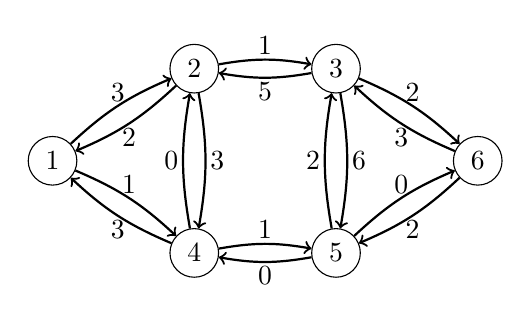
\begin{tikzpicture}[scale=0.9,label distance=-2mm]
\node[draw, circle] (1) at (1,1.3) {$1$};
\node[draw, circle] (2) at (3,2.6) {$2$};
\node[draw, circle] (3) at (5,2.6) {$3$};
\node[draw, circle] (4) at (7,1.3) {$6$};
\node[draw, circle] (5) at (3,0) {$4$};
\node[draw, circle] (6) at (5,0) {$5$};

\path[draw,thick,->] (1) edge [bend left=10] node[font=\small,label=3] {} (2);
\path[draw,thick,->] (2) edge [bend left=10] node[font=\small,label=below:2] {} (1);
\path[draw,thick,->] (2) edge [bend left=10] node[font=\small,label=1] {} (3);
\path[draw,thick,->] (3) edge [bend left=10] node[font=\small,label=below:5] {} (2);
\path[draw,thick,->] (3) edge [bend left=10] node[font=\small,label=2] {} (4);
\path[draw,thick,->] (4) edge [bend left=10] node[font=\small,label=below:3] {} (3);
\path[draw,thick,->] (1) edge [bend left=10] node[font=\small,label=1] {} (5);
\path[draw,thick,->] (5) edge [bend left=10] node[font=\small,label=below:3] {} (1);
\path[draw,thick,->] (5) edge [bend left=10] node[font=\small,label=1] {} (6);
\path[draw,thick,->] (6) edge [bend left=10] node[font=\small,label=below:0] {} (5);
\path[draw,thick,->] (6) edge [bend left=10] node[font=\small,label=0] {} (4);
\path[draw,thick,->] (4) edge [bend left=10] node[font=\small,label=below:2] {} (6);
\path[draw,thick,->] (5) edge [bend left=10] node[font=\small,label=left:0] {} (2);
\path[draw,thick,->] (2) edge [bend left=10] node[font=\small,label=right:3] {} (5);
\path[draw,thick,->] (3) edge [bend left=10] node[font=\small,label=right:6] {} (6);
\path[draw,thick,->] (6) edge [bend left=10] node[font=\small,label=left:2] {} (3);
\end{tikzpicture}
\end{center}
\end{samepage}

Maksimivirtaus tulee valmiiksi
lisäämällä virtausta vielä polkujen $1 \rightarrow 2 \rightarrow 3 \rightarrow 6$ ja
$1 \rightarrow 4 \rightarrow 5 \rightarrow 3 \rightarrow 6$ avulla.
Molemmat polut tuottavat 1 yksikön lisää virtausta,
ja lopullinen verkko on seuraava:

\begin{center}
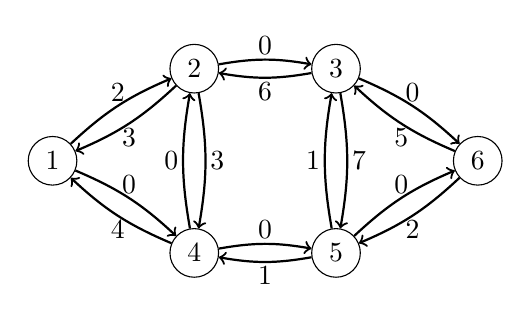
\begin{tikzpicture}[scale=0.9,label distance=-2mm]
\node[draw, circle] (1) at (1,1.3) {$1$};
\node[draw, circle] (2) at (3,2.6) {$2$};
\node[draw, circle] (3) at (5,2.6) {$3$};
\node[draw, circle] (4) at (7,1.3) {$6$};
\node[draw, circle] (5) at (3,0) {$4$};
\node[draw, circle] (6) at (5,0) {$5$};

\path[draw,thick,->] (1) edge [bend left=10] node[font=\small,label=2] {} (2);
\path[draw,thick,->] (2) edge [bend left=10] node[font=\small,label=below:3] {} (1);
\path[draw,thick,->] (2) edge [bend left=10] node[font=\small,label=0] {} (3);
\path[draw,thick,->] (3) edge [bend left=10] node[font=\small,label=below:6] {} (2);
\path[draw,thick,->] (3) edge [bend left=10] node[font=\small,label=0] {} (4);
\path[draw,thick,->] (4) edge [bend left=10] node[font=\small,label=below:5] {} (3);
\path[draw,thick,->] (1) edge [bend left=10] node[font=\small,label=0] {} (5);
\path[draw,thick,->] (5) edge [bend left=10] node[font=\small,label=below:4] {} (1);
\path[draw,thick,->] (5) edge [bend left=10] node[font=\small,label=0] {} (6);
\path[draw,thick,->] (6) edge [bend left=10] node[font=\small,label=below:1] {} (5);
\path[draw,thick,->] (6) edge [bend left=10] node[font=\small,label=0] {} (4);
\path[draw,thick,->] (4) edge [bend left=10] node[font=\small,label=below:2] {} (6);
\path[draw,thick,->] (5) edge [bend left=10] node[font=\small,label=left:0] {} (2);
\path[draw,thick,->] (2) edge [bend left=10] node[font=\small,label=right:3] {} (5);
\path[draw,thick,->] (3) edge [bend left=10] node[font=\small,label=right:7] {} (6);
\path[draw,thick,->] (6) edge [bend left=10] node[font=\small,label=left:1] {} (3);
\end{tikzpicture}
\end{center}

Nyt virtausta ei pysty enää kasvattamaan,
koska verkossa ei ole mitään polkua
alkusolmusta loppusolmuun,
jossa jokaisen kaaren paino olisi positiivinen.
Niinpä algoritmi pysähtyy ja verkon maksimivirtaus on 7.

\subsubsection{Polun valinta}

Ford-Fulkersonin algoritmi pysähtyy aina,
koska jokainen polku kasvattaa virtausta verkossa.
Polun valintatapa kuitenkin vaikuttaa siihen,
kuinka tehokas algoritmi on.
Pahimmassa tapauksessa jokainen polku
lisää virtausta vain 1:llä,
jolloin algoritmi voi toimia hitaasti.

Polun valintaan on kaksi helposti toteutettavaa tapaa,
jotka varmistavat, että virtaus kasvaa nopeasti:

\textit{Edmonds-Karpin algoritmi} on
Ford-Fulkersonin algoritmin toteutus,
jossa virtausta kasvattava polku valitaan
aina niin, että siinä on mahdollisimman vähän kaaria.
Tämä onnistuu etsimällä polku leveyshaulla
alkusolmusta lähtien.
Algoritmin aikavaativuus on $O(m^2 n)$.

\textit{Skaalaava algoritmi}
asettaa minimipainon, joka on ensin alkusolmusta
lähtevien kaarten painojen summa $c$.
Joka vaiheessa verkosta etsitään
syvyyshaulla polku, jonka jokaisen kaaren paino
on vähintään minimipaino.
Aina jos kelvollista polkua ei löydy,
minimipaino jaetaan 2:lla,
kunnes lopuksi minimipaino on 1.
Algoritmin aikavaativuus on $O(m^2 \log c)$.

Käytännössä skaalaava algoritmi on mukavampi koodattava,
koska siinä riittää etsiä polku syvyyshaulla.
Kummatkin algoritmit ovat yleensä aina riittävän
nopeita ohjelmointikisoissa esiintyviin tehtäviin.

\subsubsection{Minimileikkaus}

Kun Ford-Fulkersonin algoritmi on saanut valmiiksi
maksimivirtauksen, se on tuottanut samalla minimileikkauksen.
Olkoon $A$ niiden solmujen joukko,
joihin verkossa pääsee
alkusolmusta positiivisia kaaria pitkin.
Esimerkkiverkossa $A$ sisältää solmut 1, 2 ja 4:

\begin{center}
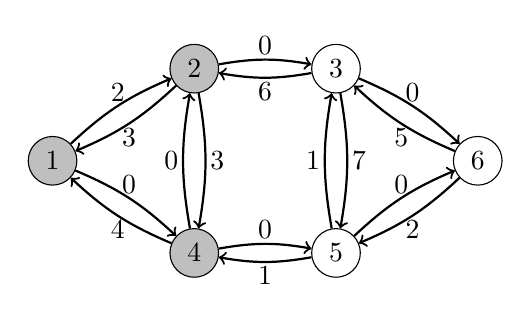
\begin{tikzpicture}[scale=0.9,label distance=-2mm]
\node[draw, circle,fill=lightgray] (1) at (1,1.3) {$1$};
\node[draw, circle,fill=lightgray] (2) at (3,2.6) {$2$};
\node[draw, circle] (3) at (5,2.6) {$3$};
\node[draw, circle] (4) at (7,1.3) {$6$};
\node[draw, circle,fill=lightgray] (5) at (3,0) {$4$};
\node[draw, circle] (6) at (5,0) {$5$};

\path[draw,thick,->] (1) edge [bend left=10] node[font=\small,label=2] {} (2);
\path[draw,thick,->] (2) edge [bend left=10] node[font=\small,label=below:3] {} (1);
\path[draw,thick,->] (2) edge [bend left=10] node[font=\small,label=0] {} (3);
\path[draw,thick,->] (3) edge [bend left=10] node[font=\small,label=below:6] {} (2);
\path[draw,thick,->] (3) edge [bend left=10] node[font=\small,label=0] {} (4);
\path[draw,thick,->] (4) edge [bend left=10] node[font=\small,label=below:5] {} (3);
\path[draw,thick,->] (1) edge [bend left=10] node[font=\small,label=0] {} (5);
\path[draw,thick,->] (5) edge [bend left=10] node[font=\small,label=below:4] {} (1);
\path[draw,thick,->] (5) edge [bend left=10] node[font=\small,label=0] {} (6);
\path[draw,thick,->] (6) edge [bend left=10] node[font=\small,label=below:1] {} (5);
\path[draw,thick,->] (6) edge [bend left=10] node[font=\small,label=0] {} (4);
\path[draw,thick,->] (4) edge [bend left=10] node[font=\small,label=below:2] {} (6);
\path[draw,thick,->] (5) edge [bend left=10] node[font=\small,label=left:0] {} (2);
\path[draw,thick,->] (2) edge [bend left=10] node[font=\small,label=right:3] {} (5);
\path[draw,thick,->] (3) edge [bend left=10] node[font=\small,label=right:7] {} (6);
\path[draw,thick,->] (6) edge [bend left=10] node[font=\small,label=left:1] {} (3);
\end{tikzpicture}
\end{center}

Nyt minimileikkauksen muodostavat ne alkuperäisen verkon kaaret,
jotka kulkevat joukosta $A$ joukon $A$ ulkopuolelle
ja joiden kapasiteetti on täysin käytetty
maksimivirtauksessa.
Tässä verkossa kyseiset kaaret ovat $2 \rightarrow 3$
ja $4 \rightarrow 5$, jotka tuottavat minimileikkauksen $6+1=7$.

Minimileikkauksen olemassaolo myös perustelee,
miksi Ford-Fulkersonin algoritmin tuottama virtaus
on suurin mahdollinen.
Tarkastellaan mitä tahansa verkon leikkausta,
jossa alkusolmu kuuluu osaan $A$,
loppusolmu kuuluu osaan $B$ ja osien välillä kulkee kaaria:

\begin{center}
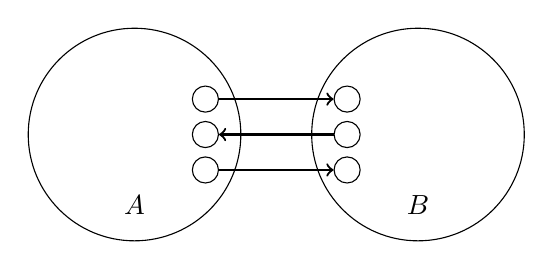
\begin{tikzpicture}[scale=0.9]
\draw (-2,0) circle (1.5);
\draw (2,0) circle (1.5);

\node at (-2,-1) {$A$};
\node at (2,-1) {$B$};

\node[draw, circle] (1) at (-1,0.5) {};
\node[draw, circle] (2) at (-1,0) {};
\node[draw, circle] (3) at (-1,-0.5) {};
\node[draw, circle] (4) at (1,0.5) {};
\node[draw, circle] (5) at (1,0) {};
\node[draw, circle] (6) at (1,-0.5) {};

\path[draw,thick,->] (1) -- (4);
\path[draw,thick,->] (5) -- (2);
\path[draw,thick,->] (3) -- (6);

\end{tikzpicture}
\end{center}

Leikkauksen paino on niiden kaarten painojen summa,
jotka kulkevat osasta $A$ osaan $B$.
Tämä on yläraja sille, kuinka suuri verkossa oleva virtaus voi olla,
koska virtauksen täytyy edetä osasta $A$ osaan $B$.
Niinpä maksimivirtaus on pienempi tai yhtä suuri kuin
mikä tahansa verkon leikkaus.

Toisaalta Ford-Fulkersonin algoritmi tuottaa virtauksen,
joka on tarkalleen yhtä suuri kuin verkossa oleva leikkaus.
Niinpä tämän virtauksen on oltava maksimivirtaus ja
vastaavasti leikkauksen on oltava minimileikkaus.

\newpage 
\section{Kaksijakoisen verkon ongelmia}

Kaksijakoisen verkon solmut voidaan jakaa
kahteen joukkoon niin, että kaikki verkon kaaret
kulkevat joukosta toiseen.
Tietyt verkko-ongelmat ovat helpompia ratkaista,
jos verkko on kaksijakoinen.
Seuraavaksi näemme, miten virtauslaskentaa voi
hyödyntää ongelmien ratkaisemisessa.

\subsection{Maksimiparitus}

Verkon paritus (\textit{matching}) muodostuu
yhdestä tai usemmasta solmuparista,
joissa kunkin parin solmujen välillä on kaari ja
sama solmu ei esiinny useassa parissa.
Maksimiparitus (\textit{maximum matching})
on puolestaan paritus, jossa parien määrä on mahdollisimman suuri.

Maksimiparituksen etsimiseen yleisessä
verkossa on olemassa polynominen algoritmi,
mutta se on hyvin monimutkainen.
Sen sijaan kaksijakoisessa verkossa
maksimiparitus on helppoa löytää
virtauslaskennan avulla.
Osoittautuu, että maksimiparituksen laskeminen vastaa
maksimivirtauksen laskemista.

Tarkastellaan esimerkkinä seuraavaa verkkoa:

\begin{center}
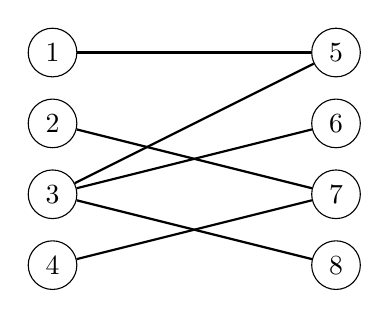
\begin{tikzpicture}[scale=0.60]
\node[draw, circle] (1) at (2,4.5) {1};
\node[draw, circle] (2) at (2,3) {2};
\node[draw, circle] (3) at (2,1.5) {3};
\node[draw, circle] (4) at (2,0) {4};
\node[draw, circle] (5) at (8,4.5) {5};
\node[draw, circle] (6) at (8,3) {6};
\node[draw, circle] (7) at (8,1.5) {7};
\node[draw, circle] (8) at (8,0) {8};

\path[draw,thick,-] (1) -- (5);
\path[draw,thick,-] (2) -- (7);
\path[draw,thick,-] (3) -- (5);
\path[draw,thick,-] (3) -- (6);
\path[draw,thick,-] (3) -- (8);
\path[draw,thick,-] (4) -- (7);
\end{tikzpicture}
\end{center}

Tässä verkossa maksimiparituksen koko on 3:
\begin{center}
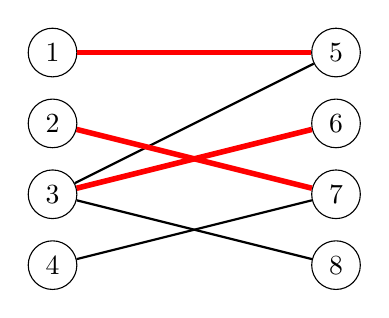
\begin{tikzpicture}[scale=0.60]
\node[draw, circle] (1) at (2,4.5) {1};
\node[draw, circle] (2) at (2,3) {2};
\node[draw, circle] (3) at (2,1.5) {3};
\node[draw, circle] (4) at (2,0) {4};
\node[draw, circle] (5) at (8,4.5) {5};
\node[draw, circle] (6) at (8,3) {6};
\node[draw, circle] (7) at (8,1.5) {7};
\node[draw, circle] (8) at (8,0) {8};

\path[draw,thick,-] (1) -- (5);
\path[draw,thick,-] (2) -- (7);
\path[draw,thick,-] (3) -- (5);
\path[draw,thick,-] (3) -- (6);
\path[draw,thick,-] (3) -- (8);
\path[draw,thick,-] (4) -- (7);

\path[draw=red,thick,-,line width=2pt] (1) -- (5);
\path[draw=red,thick,-,line width=2pt] (2) -- (7);
\path[draw=red,thick,-,line width=2pt] (3) -- (6);
\end{tikzpicture}
\end{center}

Ideana on lisätä verkkoon alkusolmu,
josta on kaari kaikkiin vasemman ryhmän solmuihin,
sekä loppusolmu,
johon on kaari kaikista oikean ryhmän solmuista.
Lisäksi ryhmien väliset kaaret muutetaan
johtamaan vasemmasta ryhmästä oikeaan.
Jokaisen kaaren kapasiteettina on 1.

Esimerkissä tuloksena on seuraava verkko:

\begin{center}
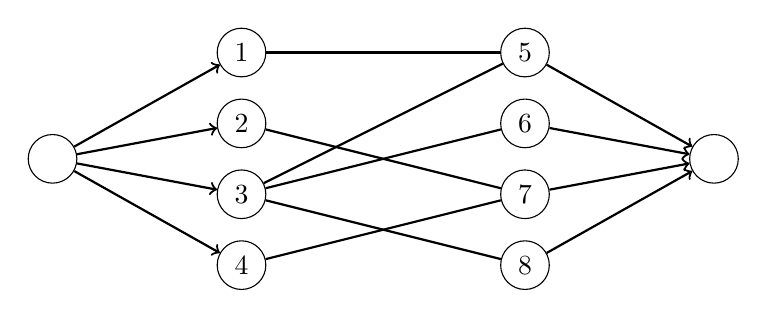
\begin{tikzpicture}[scale=0.60]
\node[draw, circle] (1) at (2,4.5) {1};
\node[draw, circle] (2) at (2,3) {2};
\node[draw, circle] (3) at (2,1.5) {3};
\node[draw, circle] (4) at (2,0) {4};
\node[draw, circle] (5) at (8,4.5) {5};
\node[draw, circle] (6) at (8,3) {6};
\node[draw, circle] (7) at (8,1.5) {7};
\node[draw, circle] (8) at (8,0) {8};

\node[draw, circle] (a) at (-2,2.25) {\phantom{0}};
\node[draw, circle] (b) at (12,2.25) {\phantom{0}};

\path[draw,thick,-] (1) -- (5);
\path[draw,thick,-] (2) -- (7);
\path[draw,thick,-] (3) -- (5);
\path[draw,thick,-] (3) -- (6);
\path[draw,thick,-] (3) -- (8);
\path[draw,thick,-] (4) -- (7);

\path[draw,thick,->] (a) -- (1);
\path[draw,thick,->] (a) -- (2);
\path[draw,thick,->] (a) -- (3);
\path[draw,thick,->] (a) -- (4);
\path[draw,thick,->] (5) -- (b);
\path[draw,thick,->] (6) -- (b);
\path[draw,thick,->] (7) -- (b);
\path[draw,thick,->] (8) -- (b);
\end{tikzpicture}
\end{center}

Tämän verkon maksimivirtaus on
alkuperäisen verkon maksimiparitus,
koska jokainen virtausta lisäävä polku
verkossa ottaa mukaan yhden uuden parin.
Tässä tapauksessa maksimivirtaus on 3,
joten maksimiparitus on myös 3.

\subsection{Hallin lause}

Hallin lause antaa ehdon, milloin kaksijakoiseen
verkkoon voidaan muodostaa paritus,
joka sisältää kaikki toisen puolen solmut.
Jos kummallakin puolella on yhtä monta solmua,
Hallin lause kertoo, voidaanko muodostaa
täydellinen paritus (\textit{perfect matching}),
jossa kaikki solmut paritetaan keskenään.

Oletetaan, että haluamme muodostaa parituksen,
johon kuuluvat kaikki vasemman puolen solmut.
Olkoon $X$ jokin joukko vasemman puolen solmuja
ja joukko $f(X)$ ne oikean puolen solmut,
jotka ovat yhteydessä joukon $X$ solmuihin.
Hallin lauseen mukaan paritus on mahdollinen
tarkalleen silloin,
kun mille tahansa joukolle $X$ pätee $|X| \le |f(X)|$.

Tarkastellaan Hallin lauseen esimerkkiverkossa.
Valitaan ensin $X=\{1,3\}$, jolloin $f(X)=\{5,6,8\}$:

\begin{center}
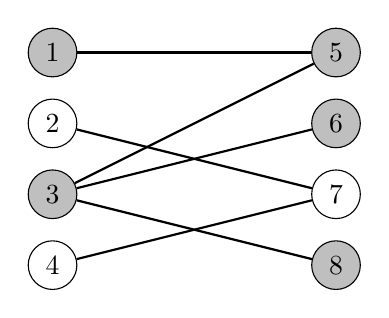
\begin{tikzpicture}[scale=0.60]
\node[draw, circle, fill=lightgray] (1) at (2,4.5) {1};
\node[draw, circle] (2) at (2,3) {2};
\node[draw, circle, fill=lightgray] (3) at (2,1.5) {3};
\node[draw, circle] (4) at (2,0) {4};
\node[draw, circle, fill=lightgray] (5) at (8,4.5) {5};
\node[draw, circle, fill=lightgray] (6) at (8,3) {6};
\node[draw, circle] (7) at (8,1.5) {7};
\node[draw, circle, fill=lightgray] (8) at (8,0) {8};

\path[draw,thick,-] (1) -- (5);
\path[draw,thick,-] (2) -- (7);
\path[draw,thick,-] (3) -- (5);
\path[draw,thick,-] (3) -- (6);
\path[draw,thick,-] (3) -- (8);
\path[draw,thick,-] (4) -- (7);
\end{tikzpicture}
\end{center}

Tämä täyttää Hallin lauseen ehdon, koska $|X|=2$ ja $|f(X)|=3$.
Valitaan sitten $X=\{2,4\}$, jolloin $f(X)=\{7\}$:

\begin{center}
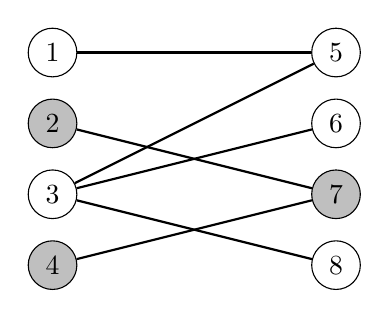
\begin{tikzpicture}[scale=0.60]
\node[draw, circle] (1) at (2,4.5) {1};
\node[draw, circle, fill=lightgray] (2) at (2,3) {2};
\node[draw, circle] (3) at (2,1.5) {3};
\node[draw, circle, fill=lightgray] (4) at (2,0) {4};
\node[draw, circle] (5) at (8,4.5) {5};
\node[draw, circle] (6) at (8,3) {6};
\node[draw, circle, fill=lightgray] (7) at (8,1.5) {7};
\node[draw, circle] (8) at (8,0) {8};

\path[draw,thick,-] (1) -- (5);
\path[draw,thick,-] (2) -- (7);
\path[draw,thick,-] (3) -- (5);
\path[draw,thick,-] (3) -- (6);
\path[draw,thick,-] (3) -- (8);
\path[draw,thick,-] (4) -- (7);
\end{tikzpicture}
\end{center}

Tässä tapauksessa $|X|=2$ ja $|f(X)|=1$, joten Hallin lauseen ehto
ei pidä paikkaansa.
Tämä tarkoittaa, että ei ole mahdollista muodostaa paritusta,
jossa ovat mukana kaikki vasemman puolen solmut.

Jos Hallin lauseen ehto ei päde, osajoukko $X$
kertoo syyn sille, miksi paritusta ei voi muodostaa.
Koska $X$ sisältää enemmän solmuja kuin $f(X)$,
kaikille $X$:n solmuille ei riitä paria oikealta.
Esimerkiksi yllä olevassa verkossa sekä solmu 2 että solmu 4 tulisi
yhdistää solmuun 7, mutta tämä ei ole mahdollista.

\subsection{Königin lause}

Solmupeite (\textit{vertex cover}) on sellainen joukko
verkon solmuja, että jokaisesta verkon kaaresta ainakin
toinen kaaren päätesolmuista kuuluu joukkoon.
Pienin solmupeite (\textit{minimum vertex cover})
on solmupeite, jossa solmujen määrä on pienin mahdollinen.

Yleisessä verkossa pienimmän solmupeitteen etsiminen
on NP-vaikea ongelma eikä siihen tunneta mitään tehokasta
algoritmia.
Kuitenkin kaksijakoisessa verkossa ongelma ratkeaa tehokkaasti,
koska Königin lauseen nojalla pienin solmupeite on yhtä suurin
kuin maksimiparitus.

Esimerkiksi seuraavan verkon maksimiparituksen koko on 3:

\begin{center}
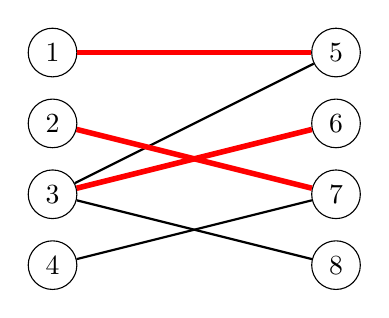
\begin{tikzpicture}[scale=0.60]
\node[draw, circle] (1) at (2,4.5) {1};
\node[draw, circle] (2) at (2,3) {2};
\node[draw, circle] (3) at (2,1.5) {3};
\node[draw, circle] (4) at (2,0) {4};
\node[draw, circle] (5) at (8,4.5) {5};
\node[draw, circle] (6) at (8,3) {6};
\node[draw, circle] (7) at (8,1.5) {7};
\node[draw, circle] (8) at (8,0) {8};

\path[draw,thick,-] (1) -- (5);
\path[draw,thick,-] (2) -- (7);
\path[draw,thick,-] (3) -- (5);
\path[draw,thick,-] (3) -- (6);
\path[draw,thick,-] (3) -- (8);
\path[draw,thick,-] (4) -- (7);

\path[draw=red,thick,-,line width=2pt] (1) -- (5);
\path[draw=red,thick,-,line width=2pt] (2) -- (7);
\path[draw=red,thick,-,line width=2pt] (3) -- (6);
\end{tikzpicture}
\end{center}

Niinpä myös pienimmän solmupeitteen koko on 3.
Solmupeite voidaan muodostaa valitsemalla siihen
solmut $\{1,3,7\}$:

\begin{center}
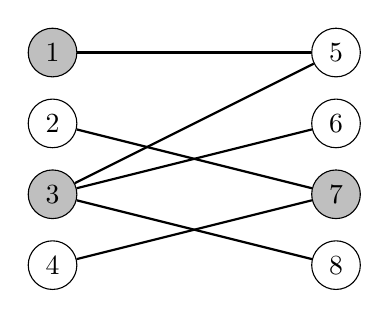
\begin{tikzpicture}[scale=0.60]
\node[draw, circle, fill=lightgray] (1) at (2,4.5) {1};
\node[draw, circle] (2) at (2,3) {2};
\node[draw, circle, fill=lightgray] (3) at (2,1.5) {3};
\node[draw, circle] (4) at (2,0) {4};
\node[draw, circle] (5) at (8,4.5) {5};
\node[draw, circle] (6) at (8,3) {6};
\node[draw, circle, fill=lightgray] (7) at (8,1.5) {7};
\node[draw, circle] (8) at (8,0) {8};

\path[draw,thick,-] (1) -- (5);
\path[draw,thick,-] (2) -- (7);
\path[draw,thick,-] (3) -- (5);
\path[draw,thick,-] (3) -- (6);
\path[draw,thick,-] (3) -- (8);
\path[draw,thick,-] (4) -- (7);
\end{tikzpicture}
\end{center}

Pienin solmupeite voidaan muodostaa aina niin,
että jokaisesta maksimiparituksen solmuparista
valitaan toinen solmuista peitteeseen.

Königin lauseen avulla ratkeaa myös toinen verkko-ongelma:
Riippumaton joukko (\textit{independent set}) on joukko
verkon solmuja, jossa minkään kahden solmun välillä ei ole kaarta.
Suurin riippumaton joukko (\textit{maximum independent set})
taas on riippumaton joukko, jossa on mahdollisimman paljon solmuja.

Suurin riippumaton joukko muodostuu valitsemalla
kaikki solmut, jotka \textit{eivät} kuulu pienimpään
solmupeitteeseen. Esimerkiksi yllä olevassa verkossa
suurin riippumaton joukko on seuraava:

\begin{center}
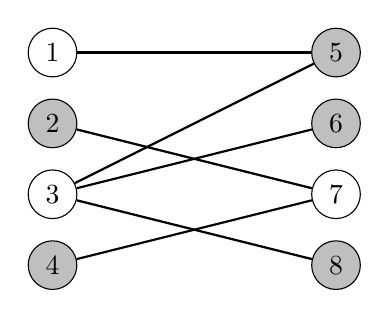
\begin{tikzpicture}[scale=0.60]
\node[draw, circle] (1) at (2,4.5) {1};
\node[draw, circle, fill=lightgray] (2) at (2,3) {2};
\node[draw, circle] (3) at (2,1.5) {3};
\node[draw, circle, fill=lightgray] (4) at (2,0) {4};
\node[draw, circle, fill=lightgray] (5) at (8,4.5) {5};
\node[draw, circle, fill=lightgray] (6) at (8,3) {6};
\node[draw, circle] (7) at (8,1.5) {7};
\node[draw, circle, fill=lightgray] (8) at (8,0) {8};

\path[draw,thick,-] (1) -- (5);
\path[draw,thick,-] (2) -- (7);
\path[draw,thick,-] (3) -- (5);
\path[draw,thick,-] (3) -- (6);
\path[draw,thick,-] (3) -- (8);
\path[draw,thick,-] (4) -- (7);
\end{tikzpicture}
\end{center}


\subsection{Polkujoukko}

Maksimivirtauksen avulla voi myös etsiä
suurimman polkujoukon, jossa jokainen polku alkaa
alkusolmusta ja päättyy loppusolmuun
ja polut eivät mene päällekkäin missään vaiheessa.

Tarkastellaan ensin tilannetta,
jossa samaa kaarta saa käyttää vain yhdessä
polussa mutta samaa solmua saa käyttää monessa polussa.

Nyt esimerkiksi verkossa
\\
\begin{center}
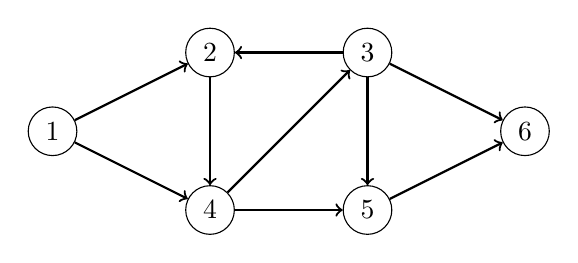
\begin{tikzpicture}
\node[draw, circle] (1) at (1,2) {$1$};
\node[draw, circle] (2) at (3,3) {$2$};
\node[draw, circle] (3) at (5,3) {$3$};
\node[draw, circle] (4) at (3,1) {$4$};
\node[draw, circle] (5) at (5,1) {$5$};
\node[draw, circle] (6) at (7,2) {$6$};
\path[draw,thick,->] (1) -- (2);
\path[draw,thick,->] (1) -- (4);
\path[draw,thick,->] (2) -- (4);
\path[draw,thick,->] (3) -- (2);
\path[draw,thick,->] (3) -- (5);
\path[draw,thick,->] (3) -- (6);
\path[draw,thick,->] (4) -- (3);
\path[draw,thick,->] (4) -- (5);
\path[draw,thick,->] (5) -- (6);
\end{tikzpicture}
\end{center}

solmusta 1 solmuun 6 pystyy muodostamaan 2 polkua.
Tämä toteutuu valitsemalla polut
$1 \rightarrow 2 \rightarrow 4 \rightarrow 3 \rightarrow 6$
ja $1 \rightarrow 4 \rightarrow 5 \rightarrow 6$:
\\
\begin{center}
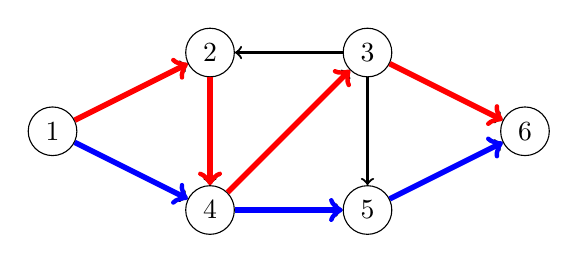
\begin{tikzpicture}
\node[draw, circle] (1) at (1,2) {$1$};
\node[draw, circle] (2) at (3,3) {$2$};
\node[draw, circle] (3) at (5,3) {$3$};
\node[draw, circle] (4) at (3,1) {$4$};
\node[draw, circle] (5) at (5,1) {$5$};
\node[draw, circle] (6) at (7,2) {$6$};
\path[draw,thick,->] (1) -- (2);
\path[draw,thick,->] (1) -- (4);
\path[draw,thick,->] (2) -- (4);
\path[draw,thick,->] (3) -- (2);
\path[draw,thick,->] (3) -- (5);
\path[draw,thick,->] (3) -- (6);
\path[draw,thick,->] (4) -- (3);
\path[draw,thick,->] (4) -- (5);
\path[draw,thick,->] (5) -- (6);

\path[draw=red,thick,->,line width=2pt] (1) -- (2);
\path[draw=red,thick,->,line width=2pt] (2) -- (4);
\path[draw=red,thick,->,line width=2pt] (4) -- (3);
\path[draw=red,thick,->,line width=2pt] (3) -- (6);

\path[draw=blue,thick,->,line width=2pt] (1) -- (4);
\path[draw=blue,thick,->,line width=2pt] (4) -- (5);
\path[draw=blue,thick,->,line width=2pt] (5) -- (6);
\end{tikzpicture}
\end{center}

Suurin polkujoukko on sama kuin verkon maksimivirtaus,
kun jokaisen kaaren paino on 1.
Tämä johtuu siitä, että painon 1 ansiosta jokaista
kaarta pystyy käyttämään vain kerran poluissa.

Tarkastellaan sitten tilannetta,
jossa myös jokaista solmua
(alku- ja loppusolmua lukuun ottamatta)
saa käyttää vain kerran.

Tavallinen tapa rajoittaa solmujen kautta
kulkemista virtauslaskennassa on korvata
jokainen solmu kahdella solmulla,
joiden välillä oleva kaari
kertoo solmun kapasiteetin.
Ensimmäinen solmuista on tulosolmu,
johon vain tulee kaaria,
ja toinen solmuista on lähtösolmu,
josta vain lähtee kaaria.

Esimerkkiverkosta tulee nyt:
\\
\begin{center}
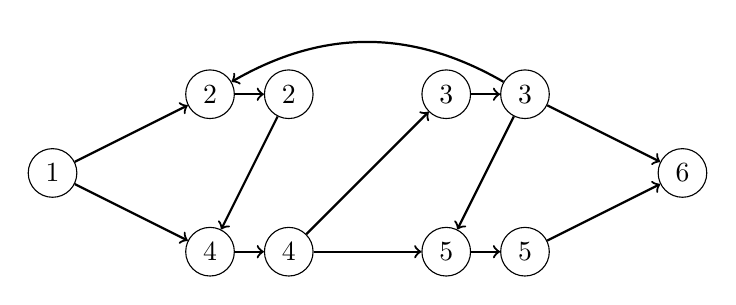
\begin{tikzpicture}
\node[draw, circle] (1) at (1,2) {$1$};

\node[draw, circle] (2a) at (3,3) {$2$};
\node[draw, circle] (3a) at (6,3) {$3$};
\node[draw, circle] (4a) at (3,1) {$4$};
\node[draw, circle] (5a) at (6,1) {$5$};

\node[draw, circle] (2b) at (4,3) {$2$};
\node[draw, circle] (3b) at (7,3) {$3$};
\node[draw, circle] (4b) at (4,1) {$4$};
\node[draw, circle] (5b) at (7,1) {$5$};

\node[draw, circle] (6) at (9,2) {$6$};

\path[draw,thick,->] (2a) -- (2b);
\path[draw,thick,->] (3a) -- (3b);
\path[draw,thick,->] (4a) -- (4b);
\path[draw,thick,->] (5a) -- (5b);

\path[draw,thick,->] (1) -- (2a);
\path[draw,thick,->] (1) -- (4a);
\path[draw,thick,->] (2b) -- (4a);
\path[draw,thick,->] (3b) edge [bend right=30] (2a);
\path[draw,thick,->] (3b) -- (5a);
\path[draw,thick,->] (3b) -- (6);
\path[draw,thick,->] (4b) -- (3a);
\path[draw,thick,->] (4b) -- (5a);
\path[draw,thick,->] (5b) -- (6);
\end{tikzpicture}
\end{center}

Maksimivirtaus tässä verkossa on
\\
\begin{center}
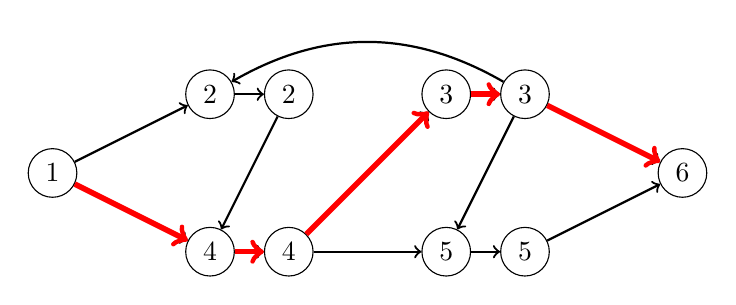
\begin{tikzpicture}
\node[draw, circle] (1) at (1,2) {$1$};

\node[draw, circle] (2a) at (3,3) {$2$};
\node[draw, circle] (3a) at (6,3) {$3$};
\node[draw, circle] (4a) at (3,1) {$4$};
\node[draw, circle] (5a) at (6,1) {$5$};

\node[draw, circle] (2b) at (4,3) {$2$};
\node[draw, circle] (3b) at (7,3) {$3$};
\node[draw, circle] (4b) at (4,1) {$4$};
\node[draw, circle] (5b) at (7,1) {$5$};

\node[draw, circle] (6) at (9,2) {$6$};

\path[draw,thick,->] (2a) -- (2b);
\path[draw,thick,->] (3a) -- (3b);
\path[draw,thick,->] (4a) -- (4b);
\path[draw,thick,->] (5a) -- (5b);

\path[draw,thick,->] (1) -- (2a);
\path[draw,thick,->] (1) -- (4a);
\path[draw,thick,->] (2b) -- (4a);
\path[draw,thick,->] (3b) edge [bend right=30] (2a);
\path[draw,thick,->] (3b) -- (5a);
\path[draw,thick,->] (3b) -- (6);
\path[draw,thick,->] (4b) -- (3a);
\path[draw,thick,->] (4b) -- (5a);
\path[draw,thick,->] (5b) -- (6);

\path[draw=red,thick,->,line width=2pt] (1) -- (4a);
\path[draw=red,thick,->,line width=2pt] (4a) -- (4b);
\path[draw=red,thick,->,line width=2pt] (4b) -- (3a);
\path[draw=red,thick,->,line width=2pt] (3a) -- (3b);
\path[draw=red,thick,->,line width=2pt] (3b) -- (6);
\end{tikzpicture}
\end{center}

mikä vastaa alkuperäisen verkon
suurinta polkujoukkoa,
jossa jokaista kaarta ja solmua saa
käyttää vain kerran:
\\
\begin{center}
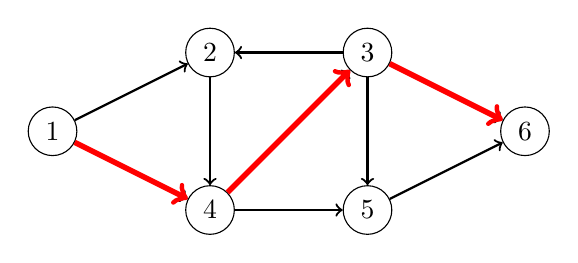
\begin{tikzpicture}
\node[draw, circle] (1) at (1,2) {$1$};
\node[draw, circle] (2) at (3,3) {$2$};
\node[draw, circle] (3) at (5,3) {$3$};
\node[draw, circle] (4) at (3,1) {$4$};
\node[draw, circle] (5) at (5,1) {$5$};
\node[draw, circle] (6) at (7,2) {$6$};
\path[draw,thick,->] (1) -- (2);
\path[draw,thick,->] (1) -- (4);
\path[draw,thick,->] (2) -- (4);
\path[draw,thick,->] (3) -- (2);
\path[draw,thick,->] (3) -- (5);
\path[draw,thick,->] (3) -- (6);
\path[draw,thick,->] (4) -- (3);
\path[draw,thick,->] (4) -- (5);
\path[draw,thick,->] (5) -- (6);

\path[draw=red,thick,->,line width=2pt] (1) -- (4);
\path[draw=red,thick,->,line width=2pt] (4) -- (3);
\path[draw=red,thick,->,line width=2pt] (3) -- (6);
\end{tikzpicture}
\end{center}
